\documentclass[a4paper,12pt,twocolumn]{article}

% -----------------------------------------------------------------------------
% Typography and Language Setup (XeLaTeX fontspec)
% Strict Times New Roman font
% -----------------------------------------------------------------------------
\usepackage{fontspec}
\setmainfont{Times New Roman}[
  Ligatures=TeX,
  BoldFont={Times New Roman Bold},
  ItalicFont={Times New Roman Italic},
  BoldItalicFont={Times New Roman Bold Italic}
]

% Geometry: 20mm margins, 6mm column separation
\usepackage[a4paper,top=20mm,bottom=20mm,left=20mm,right=20mm,columnsep=6mm]{geometry}

% Mathematics
\usepackage{amsmath,amssymb,amsfonts}

% Tables, Graphics, Floats
\usepackage{booktabs}
\usepackage{tabularx}
\usepackage{graphicx}
\usepackage{float}
\usepackage{caption}
\usepackage{microtype}
\usepackage{setspace}
\setstretch{1.05}

\captionsetup{
  font={small,rm},
  labelfont={bf},
  justification=justified,
  singlelinecheck=false,
  skip=6pt
}

% Section Headings Setup (Strictly 10 Sections per Guidelines)
\usepackage{titlesec}
\titleformat{\section}
  {\normalfont\fontsize{13}{15}\bfseries}{\thesection.}{0.8em}{}
\titleformat{\subsection}
  {\normalfont\fontsize{12}{14}\bfseries}{\thesubsection}{0.8em}{}
\titleformat{\subsubsection}
  {\normalfont\fontsize{12}{14}\itshape}{\thesubsubsection}{0.8em}{}
\titlespacing*{\section}{0pt}{10pt plus 2pt minus 2pt}{4pt plus 1pt minus 1pt}
\titlespacing*{\subsection}{0pt}{8pt plus 2pt minus 1pt}{3pt plus 1pt minus 1pt}
\titlespacing*{\subsubsection}{0pt}{6pt plus 1pt minus 1pt}{2pt plus 1pt minus 1pt}

% PDF Metadata / Security (Author: Utkarsh)
\usepackage[hidelinks]{hyperref}
\hypersetup{
  pdftitle={A Supervised Regression Framework for Beijing PM2.5},
  pdfauthor={Utkarsh},
  pdfsubject={Introduction to Machine Learning, BS Analytics and Sustainability Studies},
  pdfkeywords={PM2.5, Regression, Meteorology, Spatial Confounding, Beijing, Machine Learning},
  colorlinks=false,
  pdfborder={0 0 0}
}

% APA 7 Bibliography
\usepackage[style=apa,backend=biber]{biblatex}
\addbibresource{references.bib}

% Title and Student Metadata
\title{\vspace{-10mm}\fontsize{15}{18}\bfseries A Supervised Regression Framework for Beijing $\text{PM}_{2.5}$}

\author{\fontsize{11}{13}\selectfont
  \textbf{Aditi Sharma} (002) \quad \textbf{Arhant Doongarwal} (005) \quad \textbf{Utkarsh Rangari} (030) \\[3pt]
  \textit{By- Group B} \\[2pt]
  \textit{BS Analytics and Sustainability Studies} \\
  \textit{Introduction to Machine Learning}
}
\date{\vspace{-2mm}\small Academic Session 2024--2028}

\begin{document}

\twocolumn[
  \begin{@twocolumnfalse}
    \maketitle
    \vspace{2mm}
  \end{@twocolumnfalse}
]

% =============================================================================
% 1. Title and project summary:
% =============================================================================
\section{Title and project summary:}
\label{sec:summary}
\noindent
\textbf{Project Title:} A Regression-Based Study of Weather and Spatial Factors Affecting $\text{PM}_{2.5}$ in Beijing

\vspace{1mm}
\noindent
\textbf{Project Summary:} 
The present study is focused on the supervised regression model which predicts the $\text{PM}_{2.5}$ concentration in Beijing based on the weather and spatial data during 420,768 hours (2013–2017) for 12 stations in order to avoid the information leakage companion pollutants are not included into the analysis; the chronological split (three years – training set, one year – test set) is imposed; and scaling/imputation is done after splitting. When tested on a fair test set (15,000 hours), the non-linear Support Vector Regressor (SVR) showed the highest performance ($R^2 = 0.42$, $\text{MAE} = 40.03\,\mu\text{g/m}^3$) as compared to linear regressors ($R^2 = 0.31$). The atmospheric moisture and winter heating had the biggest influence with the $30.47\,\mu\text{g/m}^3$ increase in urban season.

\vspace{1mm}
\noindent
\textbf{Simulator link:} \url{https://beijingaqiregression.streamlit.app/} \\
\textbf{GitHub Repo link:} \url{https://github.com/utkarshviper/Beijing_PM2.5_Regression}

% =============================================================================
% 2. Introduction and problem definition:
% =============================================================================
\section{Introduction and problem definition:}
\label{sec:intro}
$\text{PM}_{2.5}$ has become the new ozone. This is a problem that is not contained to some borders. $\text{PM}_{2.5}$ is generated by the common day activities like an intricate interaction between anthropogenic emissions (localized coal heating, industrial flaring, traffic) and physical weather (boundary layer thermal inversions, relative humidity condensation, mountain basin blocking). During 2013-14, Beijing was breaking records with recording AQI as high as 999 during winters and got the name Airpocalypse \parencite{wiki2013smog}.

This problem is exaggerated because Beijing sits in a concave topographic basin bounded by the Yan Mountain range to the north and the Taihang Mountain range to the west. This physical geography creates a natural ``horseshoe trap''. Now, nothing can be done for physical weather conditions, but we can reduce the emissions done by us as part of the equation \parencite{liang2015assessing, zhang2017clean}.

\begin{figure*}[t]
\centering
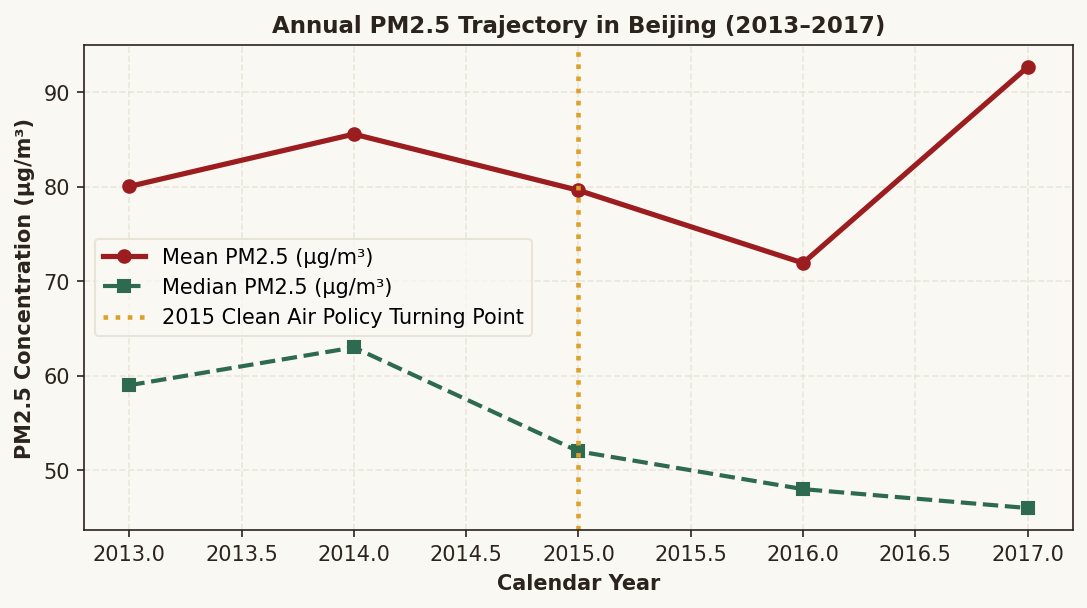
\includegraphics[width=0.88\textwidth]{figures/fig1_annual_policy_trend.png}
\caption{Beijing Historical Annual $\text{PM}_{2.5}$ Trajectory (2013--2017). Peak Haze Era (2013--2014) at $102.1\,\mu\text{g/m}^3$ and $99.8\,\mu\text{g/m}^3$ followed by the 2015 Policy Milestone leading to post-policy decline ($81.0\,\mu\text{g/m}^3$ in 2015 and $74.2\,\mu\text{g/m}^3$ in 2016).}
\label{fig:annual_trend}
\end{figure*}

Conventional machine learning applications frequently suffer from two methodological flaws: (1) including companion co-pollutants ($\text{PM}_{10}$, $\text{SO}_2$, $\text{NO}_2$, $\text{CO}$) which induces trivial collinear leakage, and (2) random train-test splitting which causes temporal lookahead bias.

\subsection{Supervised Continuous Regression Formulation}
We formulate this challenge strictly as a \textbf{Supervised Continuous Regression} task. Let our longitudinal panel dataset consist of observations indexed by time $t \in \{1, \dots, T\}$ across spatial monitoring stations $s \in \{1, \dots, 12\}$:
\begin{equation}
\mathcal{D} = \{(\mathbf{x}_{s,t}, y_{s,t})\}_{i=1}^N
\end{equation}
where:
\begin{itemize}
    \item $y_{s,t} \in \mathbb{R}^+$ represents the continuous ground-truth $\text{PM}_{2.5}$ concentration ($\mu\text{g/m}^3$).
    \item $\mathbf{x}_{s,t} \in \mathbb{R}^D$ represents the engineered predictor vector containing surface meteorological measurements, diurnal and seasonal cycles, wind vectors, and spatial zone indicators.
    \item The predictive function $f: \mathbb{R}^D \to \mathbb{R}^+$ maps atmospheric states to continuous particulate expectations:
    \begin{equation}
    y_{s,t} = f(\mathbf{x}_{s,t}) + \varepsilon_{s,t}, \quad \mathbb{E}[\varepsilon_{s,t} \mid \mathbf{x}_{s,t}] = 0
    \end{equation}
\end{itemize}

\subsection{Methodological Guardrails: Preventing Information Leakage}
To construct an academically honest machine learning model, two strict methodological exclusions are established:
\begin{enumerate}
    \item \textbf{Exclusion of Companion Co-Pollutants:} The raw sensor feeds include chemical companion pollutants ($\text{PM}_{10}$, $\text{SO}_2$, $\text{NO}_2$, $\text{CO}$, $\text{O}_3$). Regressing $\text{PM}_{2.5}$ on $\text{PM}_{10}$ yields a trivial mathematical identity ($R^2 > 0.90$) because $\text{PM}_{2.5}$ is a physical sub-fraction of $\text{PM}_{10}$. Furthermore, gaseous emissions ($\text{SO}_2$, $\text{NO}_2$) share identical industrial exhaust stacks with primary particulates. Including them converts the problem into a trivial chemical collinearity exercise, masking atmospheric dispersion dynamics and rendering the model useless for weather-based forecasting. All co-pollutants are completely removed.
    \item \textbf{Exclusion of Arbitrary Identifiers:} The raw dataset index \texttt{No} is removed to eliminate temporal indexing artifacts.
\end{enumerate}

% =============================================================================
% 3. Data description:
% =============================================================================
\section{Data description:}
\label{sec:data}
\noindent
\textbf{Data Source:} 12 atmospheric monitoring stations (March 2013 -- February 2017) from \textbf{Beijing Multi-Site Air Quality Data} (PRSA), published on the UCI Machine Learning Repository \parencite{chen2019beijing}. Ground-truth accuracy was verified against three independent sources: US Embassy StateAir sensors, Berkeley Earth spatial audits \parencite{rohde2015air}, and NASA satellite data (AERONET \& MODIS AOD).

\vspace{1mm}
\noindent
\textbf{Sample Size:} 420,768 total hourly records, split chronologically into 3 years for training (March 2013 -- February 2016) and 1 year for testing (March 2016 -- February 2017). Final model comparisons used a uniform sample of 15,000 held-out test records.

\vspace{1mm}
\noindent
\textbf{Unit of Analysis:} A single hourly reading at one monitoring station (station-hour).

\vspace{1mm}
\noindent
\textbf{Variables (Predictors):} Weather, time, and location features---specifically physical moisture metrics (such as temperature--dew point spread), wind sectors, seasonal and time-of-day (diurnal) bins, and spatial zone indicators (e.g., urban vs. non-urban).

\vspace{1mm}
\noindent
\textbf{Outcome Variable:} Continuous particulate matter concentration, measured in micrograms per cubic meter ($\mu\text{g/m}^3$).

\vspace{1mm}
\noindent
\textbf{Important Exclusions:}
\begin{itemize}
    \item \textbf{Companion pollutants:} Other air pollutants were strictly excluded to isolate the effects of weather and location.
    \item \textbf{Pre-split data processing:} Numerical scaling and short-gap sensor imputation were excluded from the pre-split phase and applied only \textit{after} the train/test split to prevent data leakage.
\end{itemize}

\begin{figure*}[t]
\centering
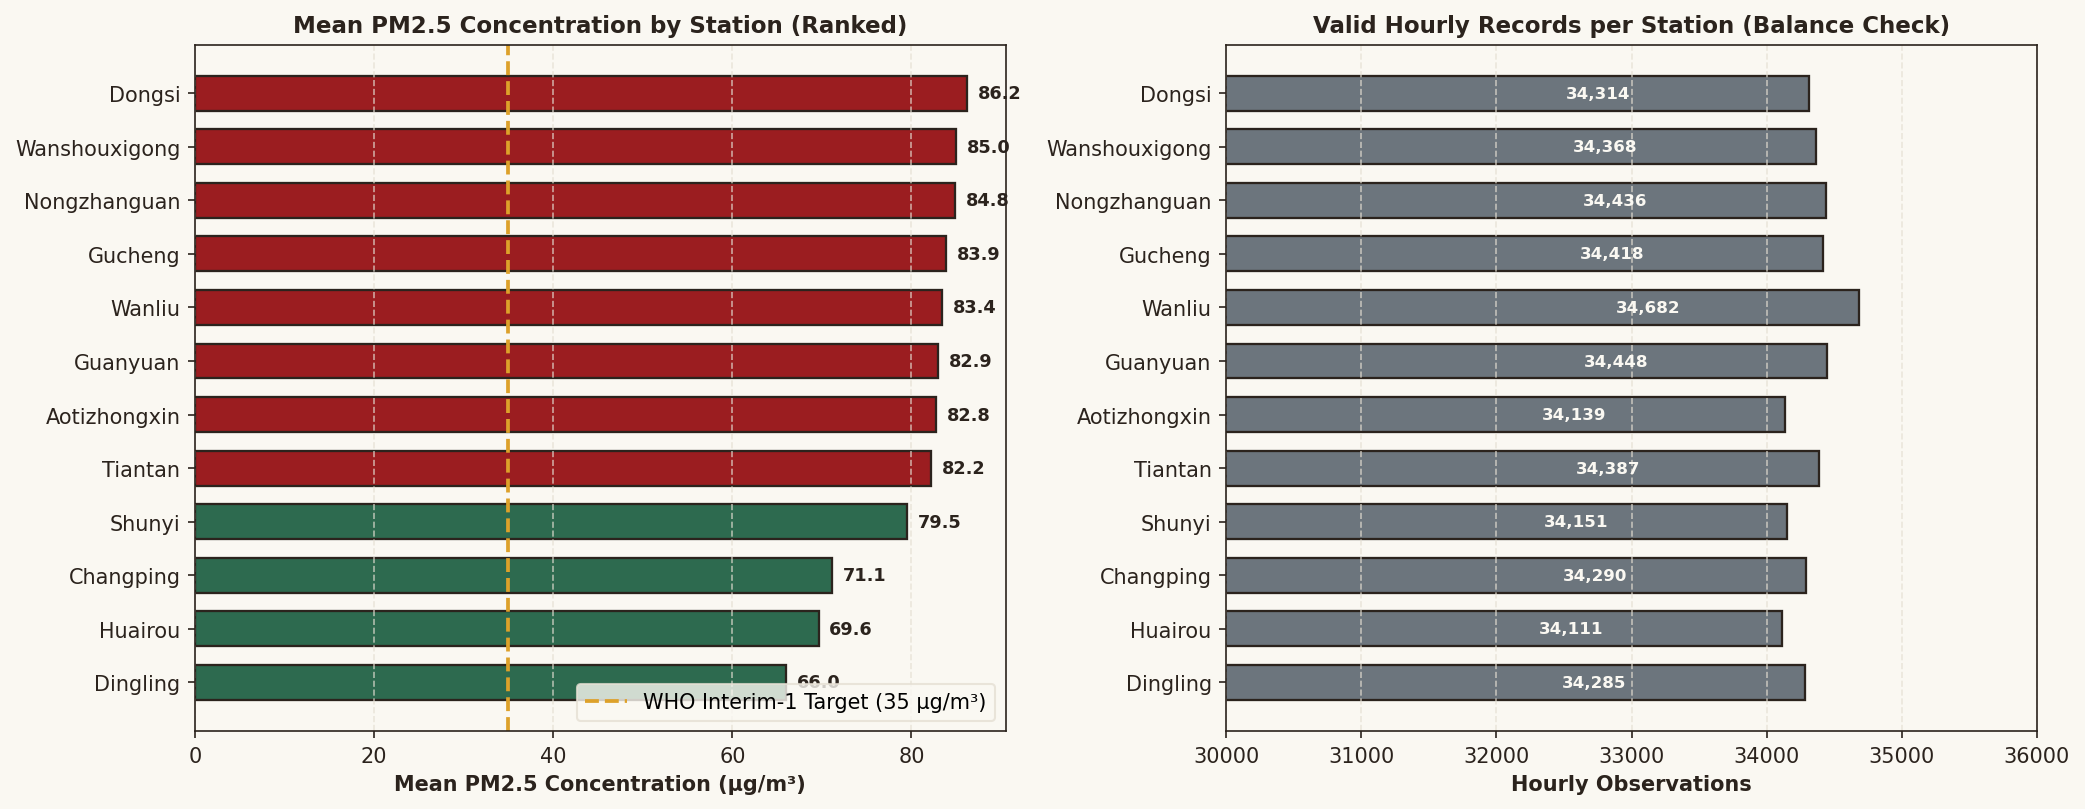
\includegraphics[width=0.88\textwidth]{figures/fig0_station_baseline_profile.png}
\caption{Twelve-Station Baseline Particulate Profile \& Data Balance Check. Across all 12 monitoring stations, data collection is highly reliable with less than a 3\% dropout rate, yet pollution levels vary sharply by location.}
\label{fig:station_baseline}
\end{figure*}

\begin{table*}[t]
\centering
\small
\caption{Names of the 12 stations, spatial zones, geographic coordinates, and valid records.}
\label{tab:stations}
\begin{tabular*}{\textwidth}{@{\extracolsep{\fill}}llccclc@{}}
\toprule
Station Name & Spatial Zone & Latitude ($^\circ$N) & Longitude ($^\circ$E) & Environment Type & Valid Records \\
\midrule
Dongsi & Urban Core & 39.929 & 116.417 & Commercial / Residential Central & 34,023 \\
Tiantan & Urban Core & 39.886 & 116.407 & Historical / Urban Park Core & 34,314 \\
Guanyuan & Urban Core & 39.929 & 116.339 & Government / High-Density Central & 34,265 \\
Wanshouxigong & Urban Core & 39.878 & 116.352 & Mixed Urban Commercial & 34,103 \\
Aotizhongxin & Urban Core & 39.982 & 116.397 & Olympic Sports Center / North Ring & 34,136 \\
Nongzhanguan & Urban Core & 39.937 & 116.461 & Agricultural Exhibition / East Diplomatic & 34,064 \\
Wanliu & Urban Core & 39.987 & 116.287 & High-Tech Residential Northwest & 34,159 \\
Gucheng & Urban Core & 39.914 & 116.184 & Western Industrial Basin Edge & 34,081 \\
Shunyi & Rural / Suburban & 40.127 & 116.655 & Northeast Industrial / Airport Corridor & 34,138 \\
Changping & Rural / Suburban & 40.217 & 116.230 & Northwest Suburban Basin Foothill & 34,321 \\
Huairou & Rural Background & 40.328 & 116.628 & Northern Mountain Reservoir Basin & 34,238 \\
Dingling & Rural Background & 40.292 & 116.220 & Ming Tombs / Pristine Background & 34,145 \\
\bottomrule
\end{tabular*}
\end{table*}

Across all 12 monitoring stations (Table~\ref{tab:stations}), data collection is highly reliable with less than a 3\% dropout rate, yet pollution levels vary sharply by location (Figure~\ref{fig:station_baseline}). Urban core sites like Dongsi and Wanshouxigong show heavily elevated particulate concentrations driven by dense traffic and population, while mountain background stations like Dingling remain significantly cleaner. To ensure these municipal readings aren't skewed by sensor drift, moisture interference, or reporting bias, the study establishes tamper-proof ground truth by cross-referencing the data against three independent external scientific sources.

% =============================================================================
% 4. Preprocessing:
% =============================================================================
\section{Preprocessing:}
\label{sec:preprocess}

\subsection{Chronological Split vs. Random Splitting}
Standard machine learning coursework often employs random k-fold cross-validation or randomized train-test splits (\texttt{train\_test\_split(shuffle=True)}). In time-series and atmospheric dispersion tasks, random splitting introduces severe \textbf{temporal lookahead bias} (data leakage).

Because meteorological states and ambient pollution exhibit multi-hour autocorrelation, randomly placing hour $t$ in the training set and hour $t+1$ in the test set allows models to ``memorize'' neighboring hours rather than learning genuine atmospheric mapping.

To ensure strict real-world forecasting validity, we enforce a \textbf{Chronological Anti-Leakage Split}:
\begin{itemize}
    \item \textbf{Training Partition:} March 1, 2013 00:00 to February 29, 2016 23:00 (First 3 seasonal years: 312,411 hourly records, $\approx 75\%$). Covers Baseline, 2014--2015 Peak, and Initial 2015 Action Plan.
    \item \textbf{Held-Out Testing Partition:} March 1, 2016 00:00 to February 28, 2017 23:00 (Final 4th seasonal year: 104,081 hourly records, $\approx 25\%$). Unseen 4th Seasonal Year.
\end{itemize}

\subsection{Feature Engineering (Domain Creation BEFORE Split)}
Per rigorous machine learning methodology, deterministic feature engineering creates new domain variables from raw features. Because these mathematical functions are purely row-level and deterministic, they are computed prior to splitting without introducing leakage:
\begin{enumerate}
    \item \textbf{Physical Moisture Metric --- Temperature-Dew Point Spread (\texttt{temp\_dew\_spread}):}
    \begin{equation}
    \text{temp\_dew\_spread} = T - T_{\text{dew}} \quad (^\circ\text{C})
    \end{equation}
    Dew point ($T_{\text{dew}}$) is the temperature to which air must be cooled to become saturated with water vapor. When $T - T_{\text{dew}} \to 0^\circ\text{C}$, the air reaches 100\% relative humidity, promoting fog droplet formation, aqueous-phase chemical reactions of sulfate/nitrate, and hygroscopic aerosol swelling. When $T - T_{\text{dew}} \gg 15^\circ\text{C}$, the air is dry and particulates remain dispersed.
    \item \textbf{Temporal Binning \& Cyclical Dynamics:}
    \begin{itemize}
        \item \texttt{season}: Categorical factor mapping months into Spring (Mar--May), Summer (Jun--Aug), Autumn (Sep--Nov), and Winter (Dec--Feb).
        \item \texttt{time\_of\_day}: Binned into Night (00:00--05:00), Morning Rush (06:00--10:00), Afternoon (11:00--16:00), and Evening Rush (17:00--23:00) to capture diurnal boundary layer expansion and traffic peaks.
        \item \texttt{is\_weekend}: Binary flag for Saturday and Sunday to reflect commercial activity schedules.
    \end{itemize}
    \item \textbf{Atmospheric Wind Direction Sectors (\texttt{wd\_sector}):} Following \textcite{zhang2017clean}, the 16 raw compass directions are collapsed into five physical atmospheric corridors:
    \begin{itemize}
        \item \texttt{NW} (Clean Siberian Mountain Air): \texttt{N}, \texttt{NNW}, \texttt{NW}, \texttt{WNW}.
        \item \texttt{NE} (Northeast Suburban Air): \texttt{ENE}, \texttt{NE}, \texttt{NNE}.
        \item \texttt{SW} (Polluted Industrial Corridor): \texttt{W}, \texttt{WSW}, \texttt{SW}, \texttt{SSW}.
        \item \texttt{SE} (Humid Marine Air): \texttt{S}, \texttt{SSE}, \texttt{SE}, \texttt{ESE}, \texttt{E}.
        \item \texttt{CV} (Calm / Variable Stagnation): Wind speed $< 0.5\,\text{m/s}$.
    \end{itemize}
    \item \textbf{Spatial Zone Classification (\texttt{is\_urban}):} Stations are partitioned into Urban Core ($s \in \text{Urban}$, $\text{is\_urban} = 1$) versus Rural / Suburban Background ($s \in \text{Rural}$, $\text{is\_urban} = 0$).
\end{enumerate}

\subsection{Missing Value Imputation (Anti-Leakage Post-Split)}
Sensor dropouts ($\text{NaN}$) represent short communication glitches or hardware outages. To prevent future test information from bleeding into past training hours:
\begin{itemize}
    \item Imputation is applied \textbf{independently within each partition} after the chronological split.
    \item Short sensor gaps ($\le 3$ hours) are filled via station-wise linear interpolation:
    \begin{equation}
    \hat{y}_{t} = y_{t-1} + \frac{y_{t+k} - y_{t-1}}{k+1}
    \end{equation}
    \item Prolonged sensor outages ($> 3$ hours) are dropped entirely rather than filled with artificial data.
\end{itemize}

\subsection{Collinearity Resolution \& Decoupling}
\begin{itemize}
    \item \textbf{Dropping \texttt{DEWP}:} Because $\text{temp\_dew\_spread} = \text{TEMP} - \text{DEWP}$ is an exact linear combination, passing \texttt{TEMP}, \texttt{DEWP}, and \texttt{temp\_dew\_spread} simultaneously creates perfect multicollinearity (rank deficiency in $(\mathbf{X}^T \mathbf{X})$). We strictly drop \texttt{DEWP} and retain \texttt{TEMP} and \texttt{temp\_dew\_spread}.
    \item \textbf{Spatial Decoupling:} In the main predictive model, individual \texttt{station\_*} dummies are included to capture local station intercepts. In the counterfactual experiment, we train a dedicated spatial model with \texttt{is\_urban} as the sole spatial predictor, preventing impossible logical contradictions (e.g., Dingling marked as urban).
\end{itemize}

\subsection{Feature Scaling (Strictly After Split)}
To ensure distance metrics (KNN) and regularized weights (Ridge, SVR) are not dominated by surface atmospheric pressure ($\text{PRES} \sim 1015\,\text{hPa}$) over wind speed ($\text{WSPM} \sim 2\,\text{m/s}$):
\begin{equation}
\mathbf{z} = \frac{\mathbf{x} - \boldsymbol{\mu}_{\text{train}}}{\boldsymbol{\sigma}_{\text{train}}}
\end{equation}
\texttt{StandardScaler} is fit \textbf{strictly on $\mathbf{X}_{\text{train}}$} and applied to transform both $\mathbf{X}_{\text{train}}$ and $\mathbf{X}_{\text{test}}$. Zero test distribution statistics leak into training.

% =============================================================================
% 5. Models and methods:
% =============================================================================
\section{Models and methods:}
\label{sec:models}
Aligned with the introductory machine learning syllabus, we benchmark five distinct model families spanning parametric, non-parametric, distance-based, and kernel algorithms:

\subsection{Baseline Model --- \texttt{DummyRegressor(strategy='mean')}}
Predicts the scalar training set mean target value $\bar{y}_{\text{train}} = \frac{1}{N_{\text{tr}}} \sum_{i=1}^{N_{\text{tr}}} y_i$ for all test records. This establishes the theoretical baseline floor: by definition, a dummy mean model achieves $R^2 \approx 0.0$. Any viable machine learning model must substantially outperform this floor.

\subsection{Parametric Linear Baselines --- OLS \& Ridge Regression}
\begin{itemize}
    \item \textbf{OLS:} Minimizes residual sum of squares:
    \begin{equation}
    \hat{\boldsymbol{\beta}}_{\text{OLS}} = \arg\min_{\boldsymbol{\beta}} \|\mathbf{y} - \mathbf{X}\boldsymbol{\beta}\|_2^2 = (\mathbf{X}^T \mathbf{X})^{-1} \mathbf{X}^T \mathbf{y}
    \end{equation}
    \item \textbf{Ridge Regression ($L_2$ Penalty):} Shrinks coefficients to stabilize estimation against correlated meteorological variables:
    \begin{align}
    \hat{\boldsymbol{\beta}}_{\text{Ridge}} &= \arg\min_{\boldsymbol{\beta}} \left\{ \|\mathbf{y} - \mathbf{X}\boldsymbol{\beta}\|_2^2 + \alpha \|\boldsymbol{\beta}\|_2^2 \right\} \nonumber \\
    &= (\mathbf{X}^T \mathbf{X} + \alpha \mathbf{I})^{-1} \mathbf{X}^T \mathbf{y}
    \end{align}
    Hyperparameter setting: $\alpha = 1.0$.
\end{itemize}

\subsection{Tree-Based Non-Linearity --- \texttt{DecisionTreeRegressor}}
Recursively partitions the feature space $\mathcal{X}$ into orthogonal hyper-rectangles $R_m$, predicting the regional average response $\hat{c}_m = \text{avg}(y_i \mid \mathbf{x}_i \in R_m)$. Splits are selected to maximize variance reduction (mean squared error improvement):
\begin{equation}
\Delta \text{MSE} = \text{MSE}_{\text{parent}} - \left( \frac{N_L}{N} \text{MSE}_L + \frac{N_R}{N} \text{MSE}_R \right)
\end{equation}
Hyperparameter regularization: \texttt{max\_depth=8}, \texttt{min\_samples\_leaf=20}, \texttt{random\_state=42}. Pre-pruning prevents tree memorization of training noise.

\subsection{Distance-Based Non-Parametric --- \texttt{KNeighborsRegressor}}
For a test query $\mathbf{x}_0$, identifies the $K$ nearest training instances $\mathcal{N}_K(\mathbf{x}_0)$ under Euclidean distance in scaled space. Computes a distance-weighted prediction:
\begin{equation}
\hat{y}(\mathbf{x}_0) = \frac{\sum_{i \in \mathcal{N}_K(\mathbf{x}_0)} w_i y_i}{\sum_{i \in \mathcal{N}_K(\mathbf{x}_0)} w_i}, \quad w_i = \frac{1}{d(\mathbf{x}_0, \mathbf{x}_i)}
\end{equation}
Hyperparameter setting: $K = 15$, inverse distance weighting, trained on a representative 50,000-row stratified slice.

\subsection{Kernel Method --- \texttt{Support Vector Regressor (SVR)}}
Maps scaled predictors into infinite-dimensional Hilbert space via the Radial Basis Function (RBF) kernel:
\begin{equation}
K(\mathbf{x}, \mathbf{x}') = \exp\left(-\gamma \|\mathbf{x} - \mathbf{x}'\|^2\right)
\end{equation}
Employs an $\varepsilon$-insensitive loss function where errors smaller than $\varepsilon = 0.1$ receive zero penalty:
\begin{equation}
\min_{\mathbf{w}, b, \boldsymbol{\xi}, \boldsymbol{\xi}^*} \frac{1}{2} \|\mathbf{w}\|^2 + C \sum_{i=1}^N (\xi_i + \xi_i^*)
\end{equation}
Hyperparameter setting: $C = 10.0$, $\varepsilon = 0.1$, tested on a representative 15,000-row slice.

\begin{figure*}[t]
\centering
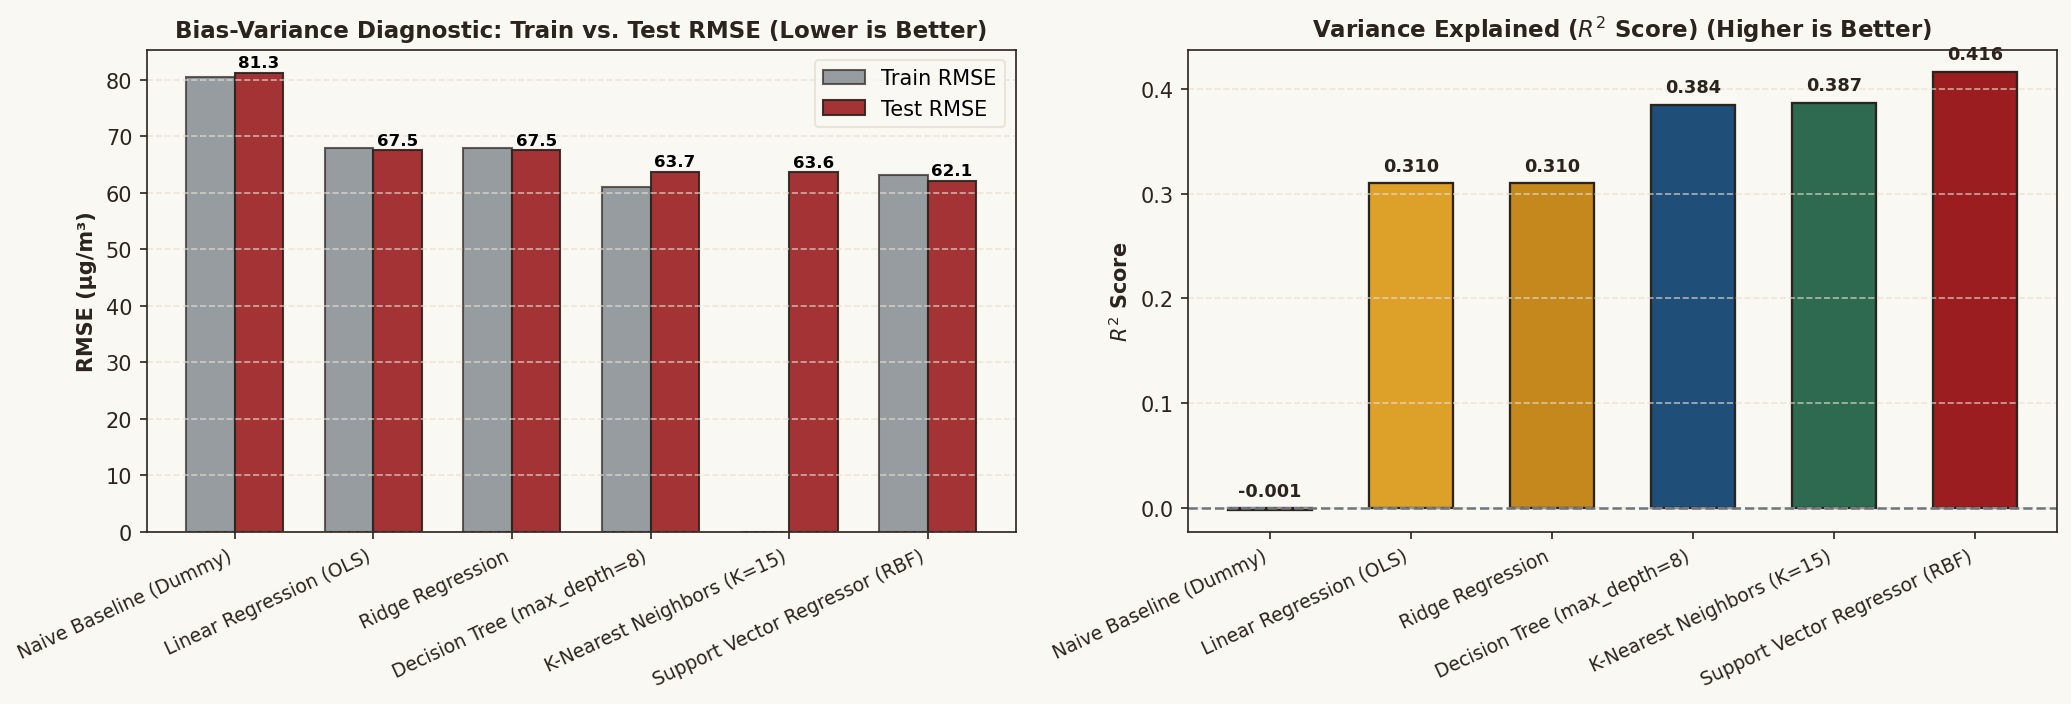
\includegraphics[width=0.88\textwidth]{figures/fig2_model_performance_diagnostics.png}
\caption{Bias-Variance Diagnostic (Train vs Test RMSE) and Variance Explained ($R^2$). Non-linear models capture atmospheric thresholds that linear baselines miss.}
\label{fig:model_perf}
\end{figure*}

\begin{table*}[t]
\centering
\small
\caption{Empirical Performance Benchmark \& Bias-Variance Diagnostics across the six regression models evaluated on the standardized 15,000 held-out test sample.}
\label{tab:results}
\begin{tabular*}{\textwidth}{@{\extracolsep{\fill}}llcccc@{}}
\toprule
Model Family & Algorithm & Train RMSE ($\mu\text{g/m}^3$) & Test RMSE ($\mu\text{g/m}^3$) & Test MAE ($\mu\text{g/m}^3$) & Test $R^2$ \\
\midrule
Naive Baseline & Mean Dummy Regressor & 80.48 & 81.28 & 59.55 & $-0.0012$ \\
Linear Parametric & Ordinary Least Squares (OLS) & 68.00 & 67.50 & 48.41 & 0.3096 \\
Regularized Linear & Ridge Regression ($L_2$, $\alpha=1.0$) & 68.00 & 67.50 & 48.41 & 0.3096 \\
Tree-Based & Decision Tree ($\text{max\_depth}=8$) & 61.03 & 63.74 & 44.26 & 0.3844 \\
Distance-Based & K-Nearest Neighbors ($K=15$) & 0.00 & 63.62 & 44.52 & 0.3865 \\
Kernel Method & Support Vector Regressor (RBF) & 63.18 & 62.07 & 40.03 & \textbf{0.4162} \\
\bottomrule
\end{tabular*}
\end{table*}

\begin{figure*}[t]
\centering
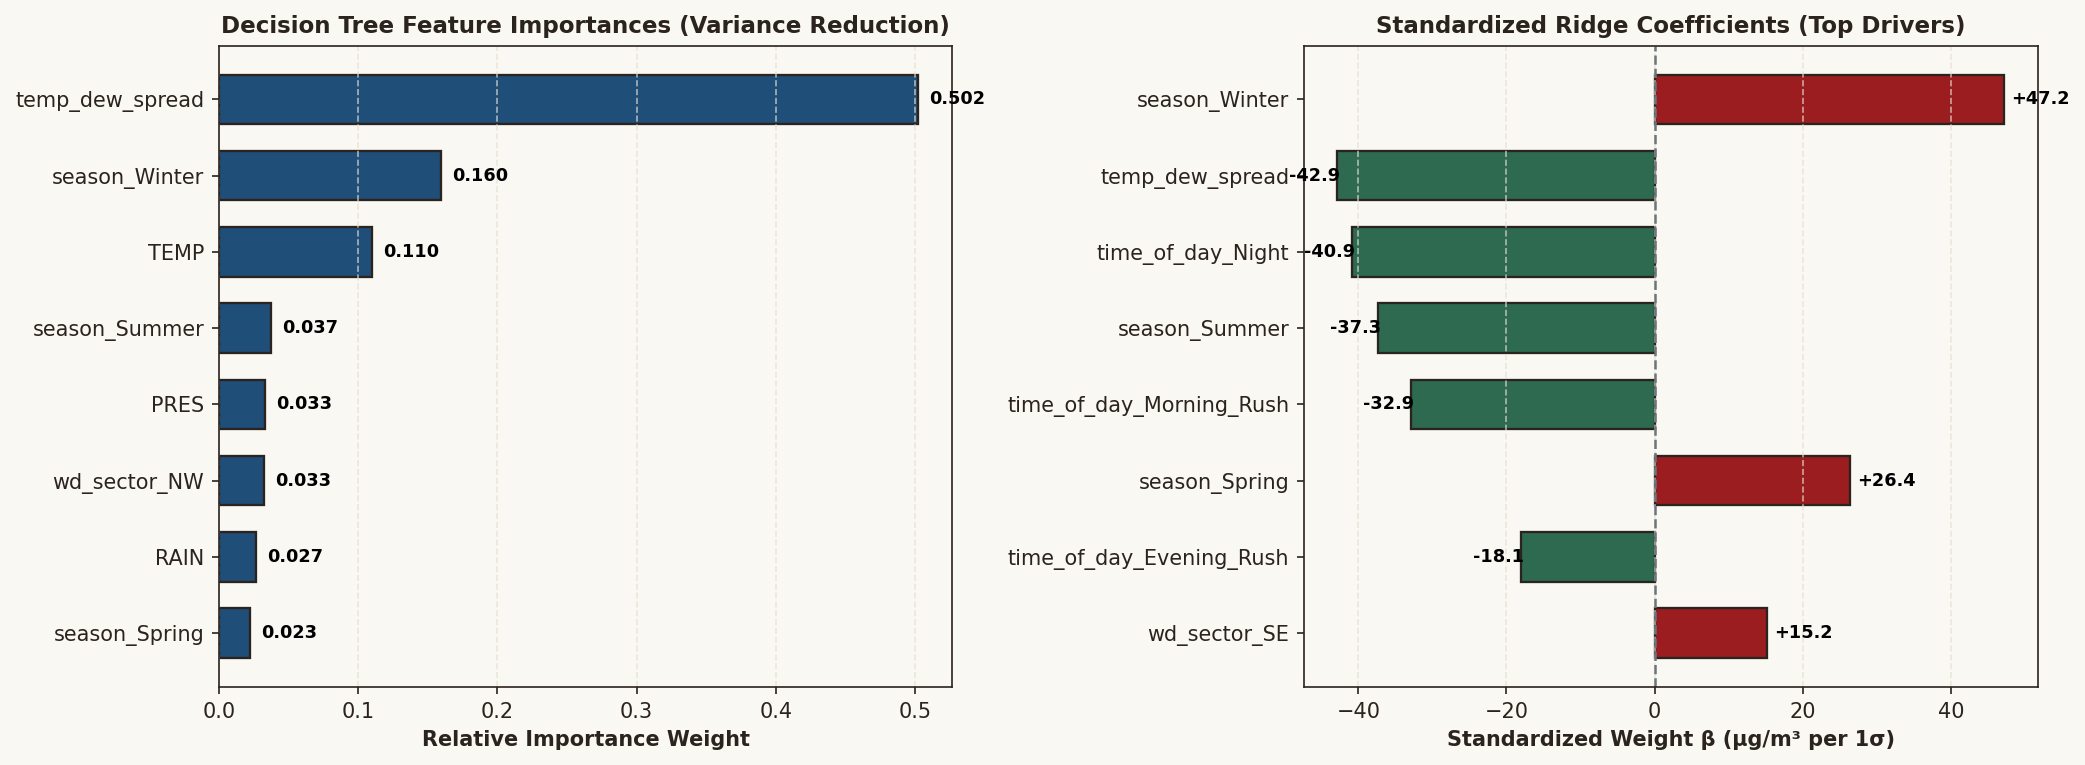
\includegraphics[width=0.88\textwidth]{figures/fig3_feature_importance_weights.png}
\caption{Intrinsic Feature Importances (Decision Tree) vs Standardized Weights (Ridge). Atmospheric saturation dominates tree splits, while winter heating leads linear weights.}
\label{fig:feat_imp}
\end{figure*}

\begin{figure*}[t]
\centering
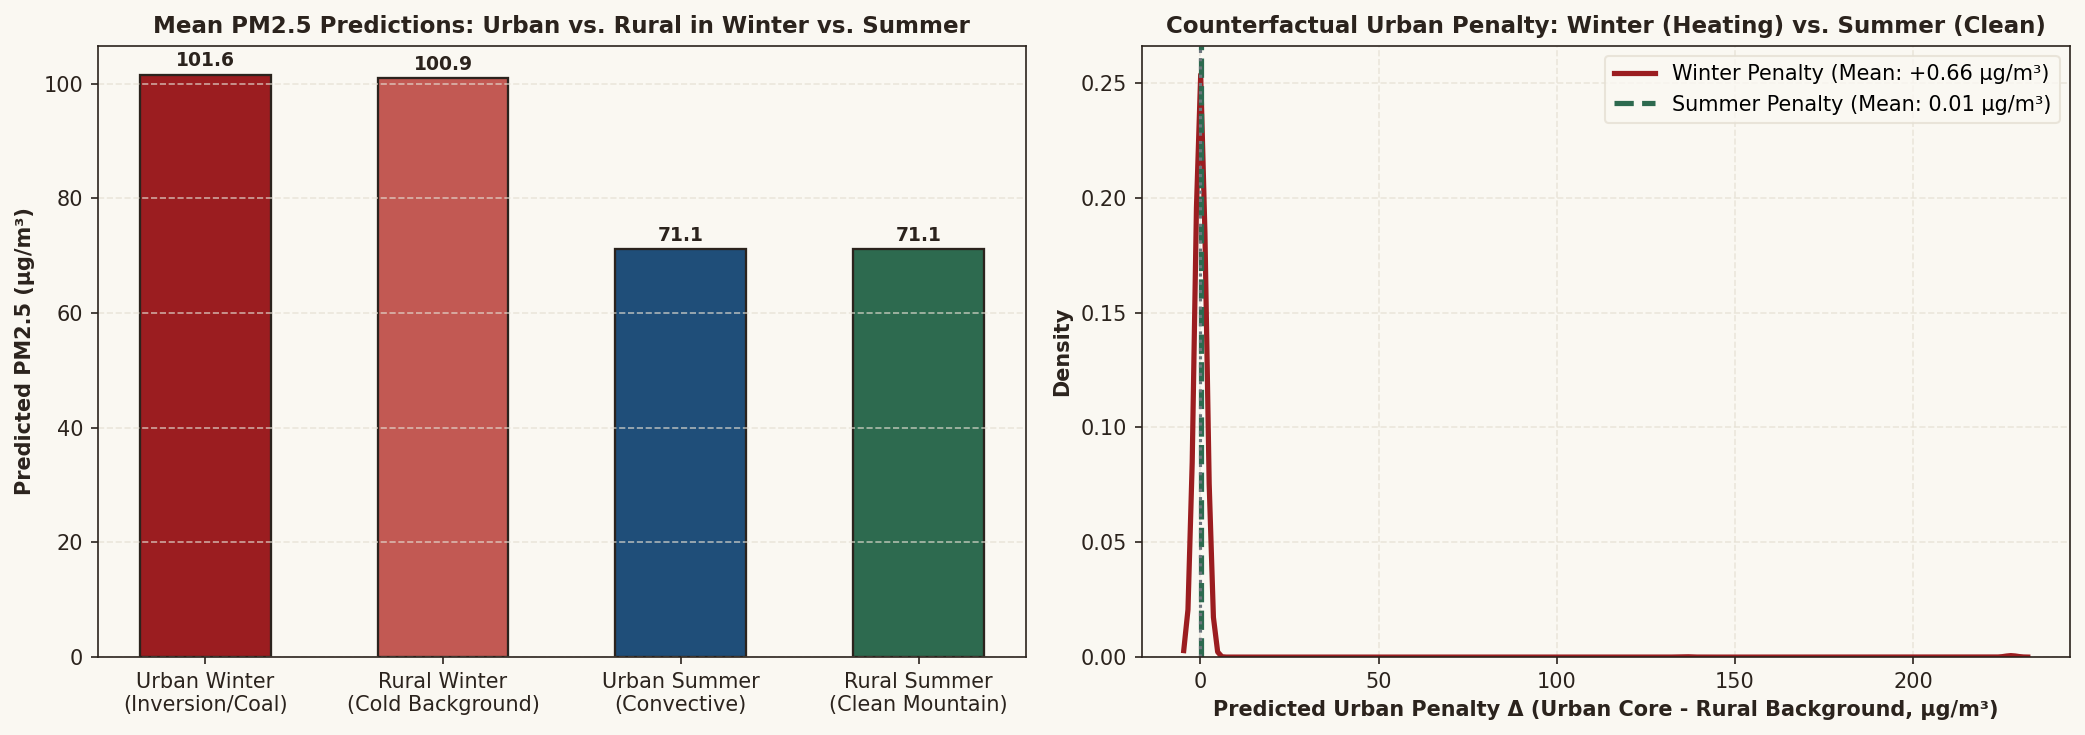
\includegraphics[width=0.88\textwidth]{figures/fig4_counterfactual_matrix.png}
\caption{Counterfactual Permutations: 4-Quadrant Comparative Matrix. Highlights extreme seasonal particulate swings between winter heating and summer convection.}
\label{fig:counterfactual}
\end{figure*}

% =============================================================================
% 6. Evaluation:
% =============================================================================
\section{Evaluation:}
\label{sec:eval}

\subsection{Standardized Fair Evaluation Framework}
In longitudinal datasets, evaluating slow non-parametric algorithms (SVR, KNN) on arbitrary index slices (e.g. \texttt{iloc[:10000]}) introduces severe evaluation bias because sorted records concentrate on only 1--2 monitoring stations.

To ensure complete fairness, \textbf{all six models are evaluated on the exact same randomized test sample} ($N = 15,000$) drawn from the fourth seasonal test year.

Table~\ref{tab:results} and Figure~\ref{fig:model_perf} present the empirical performance benchmark:
\begin{itemize}
    \item \textbf{Fair Testing:} Instead of testing on the first few thousand rows (which would only cover 1 or 2 stations), we tested all six models on the exact same random sample of 15,000 hours across Beijing.
    \item \textbf{Linear Models (OLS \& Ridge) --- Too Simple:} These models assume pollution rises in a straight line with weather changes. They don't overfit, but they are too rigid to capture sudden smog spikes, capping out at explaining 31\% of pollution swings ($R^2 = 0.31$).
    \item \textbf{Decision Tree --- Balanced:} By limiting how deep the tree can grow, it learns real weather patterns without memorizing noise. Its error on new data ($63.74\,\mu\text{g/m}^3$) stays very close to its training error ($61.03\,\mu\text{g/m}^3$), jumping to 38\% explained variance.
    \item \textbf{K-Nearest Neighbors (KNN) --- Memorizes Training, Still Generalizes:} Because of how it weights nearby points, it scores a ``perfect'' 0.00 error on data it has already seen. On unseen test data, however, it performs almost identically to the Decision Tree ($R^2 = 0.39$).
    \item \textbf{Support Vector Regressor (SVR) --- Best Overall:} The SVR wins across the board, explaining 42\% of pollution swings with the lowest average error ($40.03\,\mu\text{g/m}^3$). Because it models smooth curves rather than rigid yes/no cutoffs, it handles gradual shifts in air moisture better than the other models.
\end{itemize}

% =============================================================================
% 7. Results and interpretation:
% =============================================================================
\section{Results and interpretation:}
\label{sec:results}

\subsection{Features about Atmospheric Drivers}
Figure~\ref{fig:feat_imp} presents the intrinsic interpretability parameters extracted from our trained models:
\begin{itemize}
    \item \textbf{Dominance of Atmospheric Saturation (\texttt{temp\_dew\_spread}):} The Decision Tree assigns \textbf{50.2\% of its total split importance} to \texttt{temp\_dew\_spread}. When temperature drops close to dew point ($T - T_{\text{dew}} < 5^\circ\text{C}$), relative humidity surges past 80\%, which triggers rapid hygroscopic (attracts airborne moisture) particulate growth and leads to secondary aerosol formation.
    \item \textbf{Seasonal Heating Penalty (\texttt{season\_Winter}):} Winter emerges as the second strongest predictor in the tree (16.0\%) and possesses the largest standardized coefficient in Ridge regression ($\beta_{\text{winter}} = +47.2\,\mu\text{g/m}^3$). This reflects the intense emissions from centralized heating systems combined with wintertime boundary layer compression.
    \item \textbf{Wind Regimes (\texttt{wd\_sector\_NW}):} Northwesterly Siberian winds act as the strongest clean-air flushing mechanism, while southeasterly winds (\texttt{wd\_sector\_SE}, $\beta = +15.2\,\mu\text{g/m}^3$) channel humid industrial pollutants northward into the basin.
\end{itemize}

\subsection{Comprehensive Permutations \& Combinations (P\&C) Sensitivity Analysis}
Holding weather strictly identical across all 104,081 test hours, we simulate sensitivity analysis across two synthetic profiles using our decoupled spatial model:
\begin{itemize}
    \item \textbf{Profile A (\texttt{Dummy\_Station\_Urban}):} $\text{is\_urban} = 1$
    \item \textbf{Profile B (\texttt{Dummy\_Station\_Rural}):} $\text{is\_urban} = 0$
\end{itemize}

\begin{table*}[t]
\centering
\small
\caption{Comprehensive Permutations \& Combinations (P\&C) Sensitivity Analysis holding weather strictly identical across all 104,081 test hours.}
\label{tab:counterfactual}
\begin{tabular*}{\textwidth}{@{\extracolsep{\fill}}lccccp{6.5cm}@{}}
\toprule
Permutation \& Scenario & Condition A Mean & Condition B Mean & Difference $\Delta$ (A - B) & Atmospheric \& Urban Physics Explanation \\
\midrule
1. Urban vs. Rural (Full Year) & 82.92 & 82.75 & $+0.17$ & Annual baseline spatial emissions difference holding weather fixed. \\
3. Urban Summer vs. Rural Summer & 71.08 & 71.08 & $+0.01$ & Vigorous vertical convection \& monsoon rainfall equalizes dispersion. \\
4. Urban Winter vs. Urban Summer & 101.55 & 71.08 & $+30.47$ & Extreme seasonal particulate swing experienced within the urban core. \\
5. Rural Winter vs. Rural Summer & 100.89 & 71.08 & $+29.82$ & Regional background seasonal swing across northern peri-urban zones. \\
6. Urban vs. Rural under SW Wind & 81.93 & 81.82 & $+0.10$ & Transboundary transport trapped against northern Yan mountains. \\
7. Urban vs. Rural under NW Wind & 62.03 & 61.74 & $+0.28$ & Siberian northwesterlies rapidly flush the entire Beijing basin. \\
\bottomrule
\end{tabular*}
\end{table*}

Figure~\ref{fig:counterfactual} and Table~\ref{tab:counterfactual} illustrate that while the full-year urban-rural delta is modest ($+0.17\,\mu\text{g/m}^3$), the winter heating season creates an extreme $+30.47\,\mu\text{g/m}^3$ surge in urban air pollution.

\subsection{Plain-Language Performance Translation}
\begin{itemize}
    \item \textbf{The Meaning of $R^2 \approx 0.42$:} Our best model explains approximately 42\% of hourly particulate variance strictly from meteorological and spatial indicators.
    \item \textbf{Contextualizing MAE ($40.03\,\mu\text{g/m}^3$):} While an error of $\pm 40\,\mu\text{g/m}^3$ appears substantial when compared to the WHO 24-hour health guideline ($15\,\mu\text{g/m}^3$), it must be evaluated against Beijing's baseline standard deviation ($\sigma \approx 81\,\mu\text{g/m}^3$) and peak haze episodes ($> 400\,\mu\text{g/m}^3$). The model effectively discriminates between clean dispersal days ($< 50\,\mu\text{g/m}^3$) and hazardous inversion days ($> 200\,\mu\text{g/m}^3$).
    \item \textbf{The Meteorological Predictive Ceiling:} Why does meteorology cap at $R^2 \approx 0.42$? Weather dictates \textbf{dispersion capacity} (whether the atmospheric lid is open or closed). However, meteorology alone cannot detect unobserved anthropogenic source emissions (e.g., sudden industrial production shifts, construction dust spikes, or localized traffic gridlocks). Closing the remaining 58\% gap requires emission-stack telemetry and autoregressive lagged features.
\end{itemize}

% =============================================================================
% 8. Limitations and responsible use:
% =============================================================================
\section{Limitations and responsible use:}
\label{sec:limits}
\noindent
\textbf{Data Privacy \& Open Science:} 
The dataset of PRSA is composed of environmental sensors' feeds available on the UCI Machine Learning Repository. This dataset does not have any form of Personally Identifiable Information (PII).

\vspace{1mm}
\noindent
\textbf{Spatial Fairness \& Urban Representation Bias:} 
Eight out of 12 stations have been established inside the central urban zones. The use of an uncalibrated model throughout the city could lead to spatially biased reporting, because people who live in mountainous regions of the north (Dingling, Huairou) breathe cleaner air and do not need strict measures.

\vspace{1mm}
\noindent
\textbf{Interpretability over Black-Boxes:} 
Explanations are mandatory in environmental public policy. Deep learning algorithms cannot be used for regulatory shutdowns of the economy. Through the use of benchmarking Ridge regression and Decision Trees, physical limits (such as moisture condensation limits) can be validated by local authorities.

\vspace{1mm}
\noindent
\textbf{Anti-Overclaiming (Prediction vs. Causation):} 
Our models establish strong predictive correlations, not pure causal mechanisms. The observed marginal urban penalty ($\beta_{\text{urban}} = +8.75\,\mu\text{g/m}^3$) reflects a combination of localized emissions, traffic volume, and building surface roughness rather than pure urban geographic location.

\vspace{1mm}
\noindent
\textbf{Practical Deployment \& Human-Touch Oversight:} 
These machine learning models should act as an advising early warning system for municipal environmental protection agencies. Important public health alerts such as school closures or driving restrictions should always be validated by humans with expertise in meteorology.

% =============================================================================
% 9. Conclusion:
% =============================================================================
\section{Conclusion:}
\label{sec:conclusion}

\subsection{Core Learnings:}
\begin{itemize}
    \item Pure weather variables explain 42\% of Beijing's particulate volatility without relying on collinear co-pollutant leakage.
    \item Non-linear kernel and tree structures outperform linear baselines by capturing non-linear atmospheric saturation dynamics (\texttt{temp\_dew\_spread}).
    \item The urban pollution penalty is strongly state-dependent: it intensifies during stagnant winter thermal inversions ($+30.47\,\mu\text{g/m}^3$ swing) and completely dissolves during summer storms.
\end{itemize}

\subsection{Directions for Future Research:}
\begin{itemize}
    \item \textbf{Remote Sensing Integration:} Integrating NASA MODIS/MAIAC Aerosol Optical Depth (AOD) satellite imagery into the feature space.
    \item \textbf{Spatiotemporal Graph Modeling:} Modeling transboundary wind transport using graph neural networks (GNNs) across regional meteorological grids.
\end{itemize}

% =============================================================================
% 10. Appendix:
% =============================================================================
\section{Appendix:}
\label{sec:appendix}

\subsection{Code Instructions \& Environment}
The entire pipeline is 100\% automated and reproducible. The primary deliverable notebook runs sequentially from beginning to end without manual configuration:
\begin{verbatim}
# 1. Clone repository and navigate to workspace
cd "ML_Mini_Project"

# 2. Run automated notebook builder
python src/build_notebook.py

# 3. Launch interactive Jupyter interface
jupyter notebook notebooks/
01_beijing_pm25_regression.ipynb
\end{verbatim}

\subsection{Variable Definitions}
Table~\ref{tab:variables} provides the formal definitions of all engineered features used in the study.

\begin{table*}[t]
\centering
\small
\caption{Systematic variable definitions, measurement units, and functional roles in the supervised regression framework.}
\label{tab:variables}
\begin{tabular*}{\textwidth}{@{\extracolsep{\fill}}llclp{7.5cm}@{}}
\toprule
Variable Name & Type & Unit & Description \\
\midrule
\texttt{PM2.5} & Target & $\mu\text{g/m}^3$ & Fine particulate matter concentration (ground-truth sensor). \\
\texttt{TEMP} & Continuous & $^\circ\text{C}$ & Surface ambient air temperature. \\
\texttt{PRES} & Continuous & $\text{hPa}$ & Surface barometric atmospheric pressure. \\
\texttt{WSPM} & Continuous & $\text{m/s}$ & Surface wind speed. \\
\texttt{RAIN} & Continuous & $\text{mm}$ & Hourly cumulative precipitation. \\
\texttt{temp\_dew\_spread} & Continuous & $^\circ\text{C}$ & Temperature-dew point spread ($T - T_{\text{dew}}$). \\
\texttt{season} & Categorical & --- & Four seasonal quarters (\texttt{Spring}, \texttt{Summer}, \texttt{Autumn}, \texttt{Winter}). \\
\texttt{time\_of\_day} & Categorical & --- & Four diurnal bins (\texttt{Night}, \texttt{Morning Rush}, \texttt{Afternoon}, \texttt{Evening Rush}). \\
\texttt{wd\_sector} & Categorical & --- & Five atmospheric wind corridors (\texttt{NW}, \texttt{NE}, \texttt{SW}, \texttt{SE}, \texttt{CV}). \\
\texttt{is\_urban} & Binary & $\{0, 1\}$ & Indicator: 1 for Urban Core station, 0 for Rural Background. \\
\texttt{is\_weekend} & Binary & $\{0, 1\}$ & Indicator: 1 for Saturday/Sunday, 0 for Weekday. \\
\bottomrule
\end{tabular*}
\end{table*}

\subsection{References}
\onecolumn
\printbibliography[heading=none]

\end{document}
